
\section{Interference of Light From Multiple Slits}
\label{interference_lab}
\makelabheader %(Space for student name, etc., defined in master.tex)

\textbf{Objective}

\begin{itemize}
\item To investigate the interference of light waves as they pass through
a set of slits. 
\end{itemize}
\textbf{Apparatus}

\begin{itemize}
\item Basic optics diode laser
\item Optical bench with rotary motion sensor
\item Phototransistor for measuring light intensity (mounted on rotary motion sensor)
\item ``Multiple Slit Set'' slit accessory
%\item ``Single Slit Set'' slit accessory
\item Small plastic ruler
%\item Glass plate with sets of narrow slits
\item {\it DataStudio} 750 Interface
\end{itemize}
\textbf{Introduction}

In this laboratory you will investigate the interference of light
produced by a laser beam passing through a set of narrow, adjacent
slits. When light passes the slits each opening acts as an independent
source of waves that can overlap one another to produce a distinctive
pattern of bright and dark spots on a screen. The position of the
bright spots depends on the separation of the adjacent slits and the
wavelength of the incident light. 

You can measure this interference pattern with the setup shown below. 
(This is a \underline{top} view of the set-up.) 
A phototransistor is seated behind the narrow opening on top of the large,
metal mount sitting on a rail. The phototransistor can translate the intensity 
of the light falling on it into a voltage signal that can be read by the
computer. In addition, the phototransistor can be moved back and
forth on a rotary motion sensor that measures the position of the 
mount. These two signals can be combined to
make a graph of the intensity as a function of position.

\vspace{0.3cm}
{\centering \resizebox*{0.75\textwidth}{!}{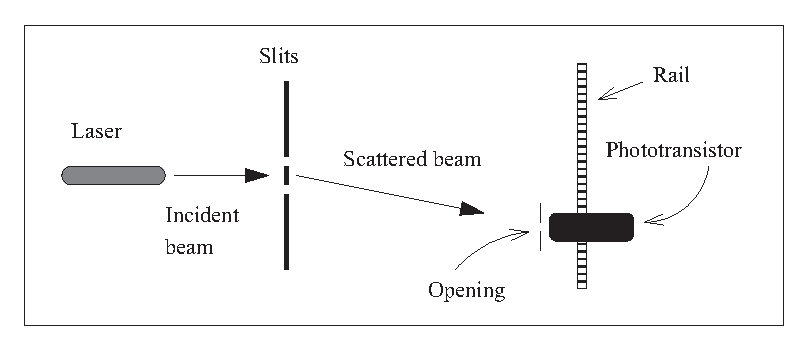
\includegraphics{interference_of_light/interference_of_light_fig1b_bw.eps}} \par}
\vspace{0.3cm}

\textbf{Activity 1: An Alternative View}

Isaac Newton believed that light was made up of small, unseen particles
that obeyed (surprisingly enough!) Newton's Laws. This view is known
as the corpuscular theory. We want to consider how this model of light
predicts different behavior from the wave theory.

\vspace{35mm}
(a) Consider a laser beam shining on a circular hole. If a beam of
light consisted of small, unseen particles that behaved as tiny billiard
balls what would you see on a screen that is downstream from the circular
hole? A sketch might be useful here.  (This question and the next one aren't hard.
They're just getting at your common sense notions about how shadows work.)
\answerspace{30mm}

(b) Now consider the same laser beam shining on a pair of narrow slits.
What would you see on a screen downstream from the slits if light
were made of corpuscles?
\answerspace{30mm}

For the questions above you should have predicted that the laser would
form a single bright spot (for part a) or two parallel lines (for part
b). The experiment you are about to perform provided compelling evidence
that Newton's corpuscular theory was wrong. 

\textbf{Activity 2: The Interference of Light }

(a) You are now ready to turn on the laser. DO NOT LOOK DIRECTLY INTO
THE BEAM OR POINT THE LASER CARELESSLY ABOUT THE ROOM. Mount the laser on the 
optical bench at the opposite end from the rotary motion sensor. Turn on the
laser and you should see the bright red spot of the beam striking
the rotary motion sensor assembly. On the ``Multiple Slit Set'' accessory, 
select a double slit of width .04 mm and separation .125 mm, marked by the number ``2''. Rotate the 
wheel so that the double slit is at the center of the opening.
%\vspace{10mm}

(b) Position the double slit about 70 cm from the phototransistor mount. Adjust 
the laser beam direction so that it falls on the double slit you have selected. 
(There are two adjustment screws on the back of the laser.) 
You should see the interference pattern on the phototransistor mount as a series of bright spots a few millimeters apart. 
%\vspace{10mm}

(c) Position the phototransistor mount so the interference pattern
is at the same height as the opening in front of the phototransistor. For best results to start with, rotate the aperture wheel on the mount to the position marked ``3'', and set the gain switch on the top of the phototransistor to ``100''. The To make accurate measurements it is important to carefully determine the geometry of your setup. Check to see if the slits and the phototransistor mount are perpendicular to the incident
laser beam.  You want to make sure the phototransistor can ``see'' as many
bright spots as possible. Carefully slide the phototransistor mount back and forth to make sure that it stays centered on the interference pattern. Then set it 
at one side of the pattern to begin the experiment.

(d) Start the ``Interference'' activity in the {\bf 132 Workshop} folder. 
When you are ready, click {\bf Start} and slowly move the phototransistor 
from one side of the slide to the other by turning the wheel on the rotary 
motion sensor. Move carefully and take about 4-5 seconds to complete the 
motion. 
As you move it, you should see a graph of the intensity reading versus the position reading. 
Click {\bf Stop} when you're done. 
The graph, called the interference pattern, should be a symmetric pattern of distinct peaks. Consult your instructor if your setup isn't working.

\pagebreak[2]
(e) In the space below, draw a good graph showing your interference pattern.  
Be sure to label your axes!
\answerspace{1.5in}

\textit{(If your instructor requests it, make a hardcopy of this graph and attach it to this unit.)}

\textbf{What's Going On?}

Let's think about why your interference pattern looks the way it does.  When the laser hits the two slits, 
light comes out of the slits in all directions all at once, as in the diagram (a) below.  
But that's a lot of light rays to keep track of, so we'll focus on just two at a time, always in the same direction, as in (b) below.
We'll define $\theta$ as the angle of the rays, where $\theta=0$ means straight ahead.  

\vspace{-0.2in}
\begin{center}
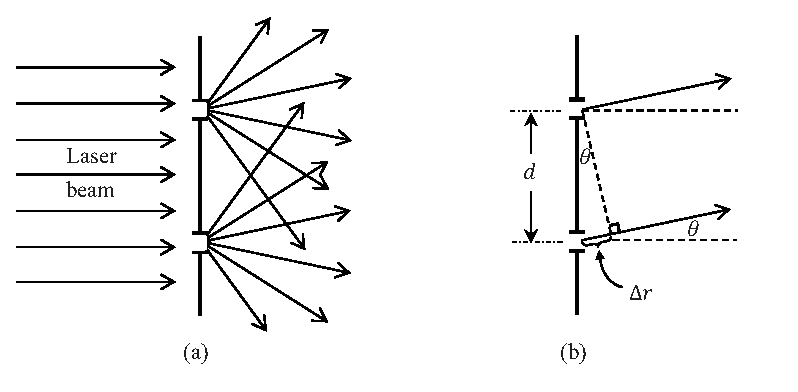
\includegraphics[width=0.63\textwidth]{interference_of_light/rays.eps}
\end{center}
\vspace{-0.2in}

The pair of rays will converge at the same spot on the screen or at the detector.  (``Wait!  How can they converge if they're parallel?!?''  Okay, they're not \textit{perfectly} parallel, but they're pretty close.  After all, the two slits are only separated by a fraction of a millimeter, and the detector is almost a meter away.  The math is way easier if we approximate the rays as parallel.)
What makes the series of bright and dark areas on the screen or at the detector is that the rays travel slightly different distances to get there.  
The difference in path length is shown on the diagram above as $\Delta r$.  

(f) For a particular angle $\theta$, if the path difference $\Delta r$ happens to be an exact integer multiple of the light's wavelength $\lambda$, will the two waves combine \textit{CONstructively} or \textit{DEstructively}?  (And does that correspond to a bright spot or a dark spot?)
\answerspace{0.5in}

(g) For a particular angle $\theta$, if the path difference $\Delta r$ happens to be an exact half-integer multiple of the light's wavelength $\lambda$ (like $0.5\lambda$ or $3.5\lambda$), will the two waves combine \textit{CONstructively} or \textit{DEstructively}?
\answerspace{0.5in}

(h) What about if the path difference $\Delta r$ happens to be something in between, like $\Delta r = 2.3\lambda$, or $0.8\lambda$? Would that place on the screen be bright? Or dark? Or something in between?
\answerspace{0.5in}

\textit{Imagine slowly increasing $\theta$, starting from zero.   As the path difference $\Delta r$ increases, the interference between the two rays oscillates between constructive and destructive, causing the oscillating pattern on your graph.}

\pagebreak[2]
\textbf{Activity 3: Determining the Wavelength of the Laser }

Now you'll use the geometry of your setup to measure the actual wavelength $\lambda$ of the light from your laser!

(a) Looking at your graph, the highest maximum is straight ahead of the slits ($\theta=0$), where $\Delta r=0$.  Does the next maximum to the right of that correspond to $\Delta r=2\lambda$?  Or $3\lambda$?  Or $19\lambda$?  Or something else?

\vspace{0.1in}
\hspace{0.8in}$\Delta r=$
\vspace{0.1in}

(b) Are the two $\theta$'s in the drawing on the last page the same?
\answerspace{0.3in}

(c) Write $\Delta r$ in terms of the distance between the slits $d$ and the the angle $\theta$.
\answerspace{0.5in}

(d) Write $\theta$ in terms of the length $L$ between the slits and the phototransistor and the horizontal distance $\Delta x$ between the two maxima.
\answerspace{0.5in}

(e) Measure $L$ carefully, using a straight edge to align objects to the scale on your tracks.  (The phototransistor is actually 25 mm behind the aperture.)  For measuring $\Delta x$ the ``Smart Tool'' on DataStudio isn't actually that smart, and won't give you enough significant digits; just read the positions of the peaks carefully from the graph, expanding the scales by dragging them if you need to.  What are your values for $L$, $\Delta x$, and $\theta$?
\answerspace{0.8in}

(f) Combine your answers for parts (a) through (e) to calculate a value for $\lambda$.  
\answerspace{1in}

(g) Does your value correspond to an accepted value for red light?
\answerspace{0.3in}

In general, we describe the interference pattern for two slits by saying that we have intensity maxima wherever 
\begin{displaymath}
d \sin \theta = m \lambda,
\end{displaymath}
where $m$ is some integer 0, 1, 2, 3, and so on.  

(h) Try calculating the wavelength of the laser light again, this time using the locations of the central maximum ($m=0$) and the one for $m=3$.  (If $m=3$ is hard to see, $m=2$ is okay too.)
\answerspace{1.0in}


\pagebreak[2]
\textbf{Activity 4: More Than Two Slits}

(a) What if, instead of two slits, you shined the laser on a series of three or four slits, all equally spaced?  Would you still see an interference pattern?  Would the spacing between maxima be the same?  What is your prediction?
\answerspace{1in}

(b) To look for any differences, you will want to have the smoothest, nicest interference pattern you can get.  Take your data again for two slits, starting with the detector at a postion fairly close to the central maximum.  When you are done, return the detector to position $x=0$ before hitting ``stop''.  

(c) Now, without deleting your previous data, switch to three slits by rotating the wheel on the slit accessory 
to ``3'', and run the pattern again.  What about the interference pattern has changed, and what has stayed the same?
\answerspace{0.8in}

(d) What happens with four slits?  Or five slits?
\answerspace{0.8in}

(e) Suppose we have three slits all a distance $d$ apart, and we draw three parallel rays from them, 1, 2, and 3.  For an angle $\theta$ at which the path difference between rays 1 and 2 just happens to be $\Delta r_{12} = \lambda$, what is the path difference $\Delta r_{13}$ between rays 1 and 3?  (A good picture might help....)
\answerspace{1.5in}

(f) Is there any angle $\theta$ at which rays 1 and 2 interfere perfectly constructively with each other,  but ray 3 interferes destructively with either of them?
\answerspace{0.4in}

\pagebreak[2]
(g) Suppose you have five rays, 1, 2, 3, 4, and 5, and suppose we consider an angle $\theta$ at which the path difference between the first two is $\Delta r_{12} = 0.8\lambda$.  What are the distances $\Delta r_{13}$, $\Delta r_{14}$, and $\Delta r_{15}$?  (Again, a good picture would help.)
\answerspace{2.5in}

(h) In the case in (g), would rays 1 and 3 interfere \textit{CON-structively} or \textit{DE-structively}?  What about rays 1 and 4?
\answerspace{0.8in}

(i) If you combined all five rays together, would the result at the detector be a place of high intensity or low intensity? 
\answerspace{0.6in}

(j) If there were only TWO slits, and you combined only TWO rays together with a path difference of $\Delta r_{12} = 0.8\lambda$, would the result at the detector be a place of high intensity or low intensity? 
\answerspace{0.6in}

(k) In general, as you increase the number of slits, do the maxima in the interference pattern become broader or narrower?  Does the maximum intensity increase or decrease?
\answerspace{0.6in}

\textbf{Activity 5: One More Thing...}

Remember the earlier discussion in Activity 1 of Newton's corpuscular theory of
light? You've taken a ton of data by now.  Does your data support Newton's theory or the wave theory of light?
Why?
\answerspace{1.0in}
